%!TEX root = ../main.tex
%%%%%%%%%%%%%%%%%%%%%%%%%%%%%%%%%%
% Links:
%
% Difficulty:
% Companies: 
%%%%%%%%%%%%%%%%%%%%%%%%%%%%%%%%%%


%\begin{figure}
%	\centering
%	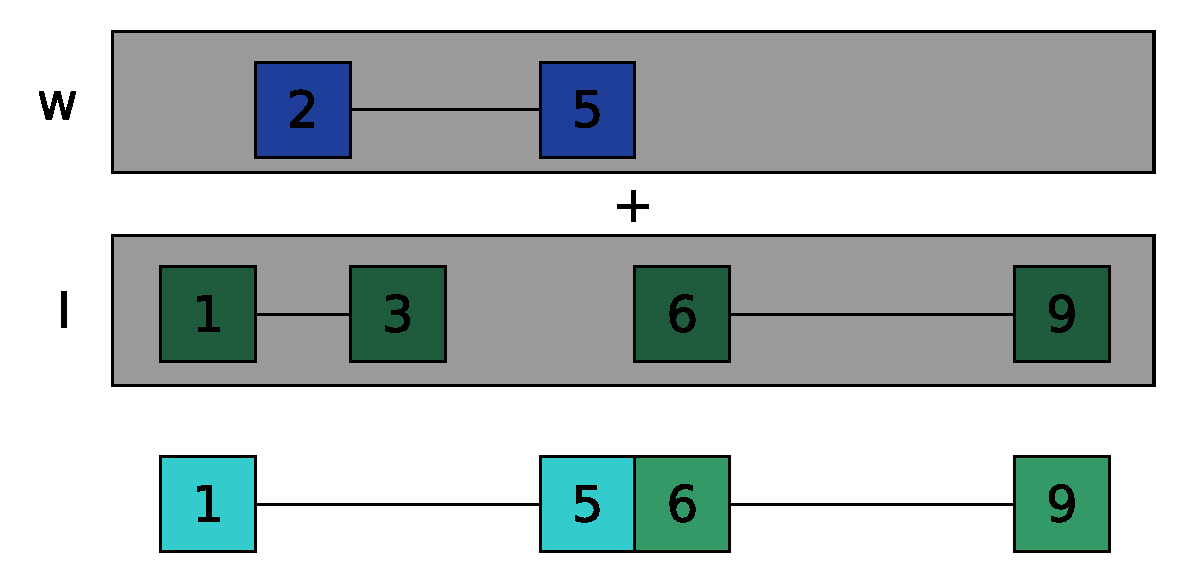
\includegraphics[width=\textwidth]{sources/merge_intervals_2/images/example1}
%	\caption[Sample short cpation]{Sample Caption}.
%	\label{fig:merge_intervals_2:example1}
%\end{figure}

\chapter{Merge Intervals}
\label{ch:merge_intervals_2}
\section*{Introduction}

\section{Problem statement}
\begin{exercise}
\label{example:merge_intervals_2:exercice1}

Given a sorted list of disjoint (non-overlapping) intervals $I$ and an interval $w$, insert $w$ into $I$ so that the resulting list still contains only disjoint intervals.
You may assume that the intervals are sorted according to their start times.

	%example1
	\begin{example}
		\label{example:merge_intervals_2:example1}
		\hfill \\
		Given $I=\{(1,3),(6,9)\}$ and $w=(2,5)$ the function returns $I'=\{(1,5),(6,9)\}$ (see Figure \ref{example:merge_intervals_2:example1}).
	\end{example}

	%example2
	\begin{example}
		\label{example:merge_intervals_2:example2}
		\hfill \\
		Given $I=\{(1,2),(3,5),(6,7),(8,10),(12,16)\}$ and $w=(4,9)$ the function returns $I'=\{(1,2),(3,10),(12,16)\}$
	\end{example}

\end{exercise}

\begin{figure}
	\centering
	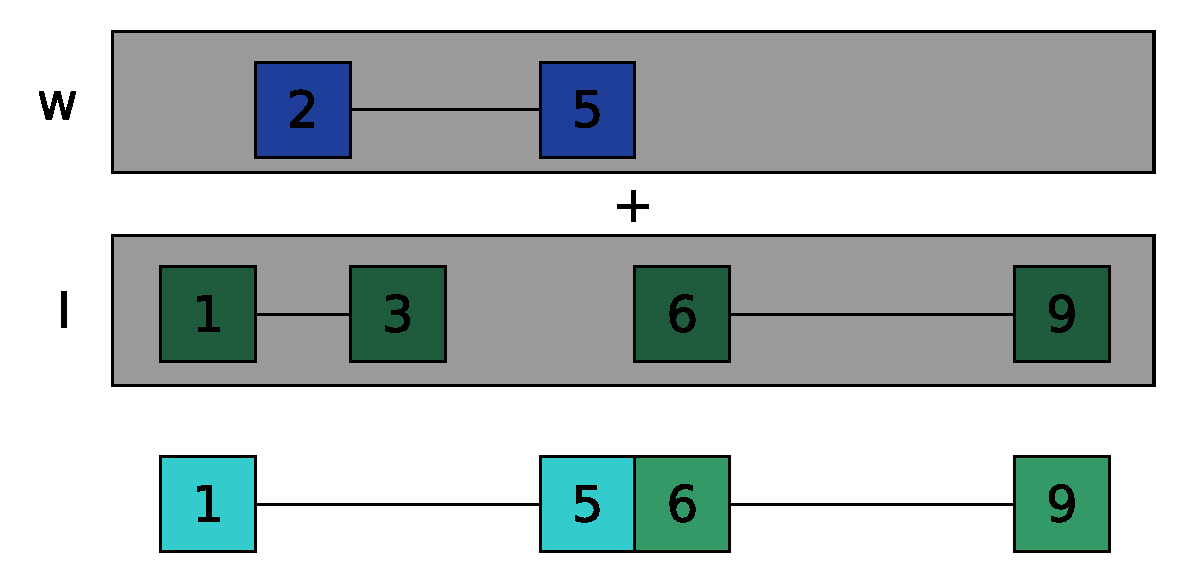
\includegraphics[width=\textwidth]{sources/merge_intervals_2/images/example1}
	\caption[Implicit graph for the Example \ref{example:merge_intervals_2:example1}.]
	{Visual representation the problem instance of Example
	\ref{example:merge_intervals_2:example1}.The \textcolor[HTML]{339966}{$\blacksquare$} green $(1,3)$ and \textcolor[HTML]{3366ff}{$\blacksquare$} blue interval $(2,5)$  are merged together into the \textcolor[HTML]{33cccc}{$\blacksquare$}cyan interval $(1,5)$ below.}
	\label{fig:merge_intervals_2:example1}
\end{figure}


\section{Clarification Questions}

\begin{QandA}
	\item 
	\begin{answered}
		\textit{}
	\end{answered}
	
\end{QandA}

\section{Discussion}
\label{merge_intervals_2:sec:discussion}


\subsection{Brute-force}
\label{merge_intervals_2:sec:bruteforce}

\begin{minipage}{\linewidth}
	\lstinputlisting[language=c++, caption={Sample Caption},label=list:merge_intervals_2]{sources/merge_intervals_2/merge_intervals_2_solution1.cpp}
\end{minipage}

